\subsection{Referring expression generation}
\label{sec:referring_expression_generation}
\subsubsection*{Setup}

Opposed to the previous experiment, where the focus lied on extracting visual features, the model is now tasked to generate referring expressions.
This is done in two setups.
The first setup uses bounding boxes as in the previous section as input, where the model needs to describe the target object of one of the bounding boxes.
In the second setup, the model is presented with the complete image and therefore also needs to accommodate to geometric information of the scene.

The bounding boxes are extracted and normalized in the same way as for the object identification task.
Since for the second setup, the images will also be passed through the feature extractors, they are normalized as well in like manner.
The referring expressions for the target object are generated using the incremental GRE-algorithm, described in Section \ref{sec:background:re}.
By this, the model needs to describe the target object with respect to the distractor objects.
There are some minor additions concerning the padding of the referring expression.
As before, the referring expression is padded to a number of three tokens, corresponding to the maximum of three attributes.
However, there are three different ways how the padding is applied.
First, the referring expression are, as usual in captioning tasks padded at the end with a specified padding token.
A problem could arise when the referring expression is not viewed as a natural language sentence, but as slots filled with tokens.
More specifically, following the GRE-algorithm, the last token in the referring expression is always the shape.
The second last token if existing describes the color, while the third last token if existing describes the size.
As soon as this sequence is padded at the end, these slots disappear.
A referring expression that only describes the shape, such as \emph{cube} will be padded to \emph{cube <pad> <pad>}, where the third last slot is filled up with the shape instead of the size.
Since this task is not focussing on producing natural language with a correct grammar, but focuses instead on extracting attributes, having a slot structure could help the model to express the extracted attributes correctly.
For this reason, the second method of padding the referring expression is prepending the referring expression with padding tokens.
By this, the positions of the slots are preserved and if not specified just filled with a padding token.
Each slot has always the same semantic value, e.g. the last slot always contains the shape of an object.
This can be done since the referring expressions are not free text, but instead the structure and the possible content is given by the dataset.
This method might help the model to learn the correct referring expressions.
% SD: Slots have the same semantic value, i.e. the last slot is the object type. We can do this because we know the structure of the descriptions in this dataset and because we hope this will help the learning. Also, we are thinking of generation based on slots.
% DK: (addressed; done)
The last variation concerns the order of producing each token.
When the referring expressions are prepended, the model would need first produce two padding tokens, before it finally can produce a much more meaningful token for the shape.
This could be difficult to learn for a model, as the longer a sequence of tokens is, the more information about the beginning of the sequence gets lost.
Even though a sequence of just three tokens may not be long enough for this factor to be a problem, we experimented to reverse the referring expression.
% SD: We... I sounds more like you are writing a lab report with casual language but here you want to be more formal.
% DK: (done)
Instead of producing for instance \emph{<pad> green sphere} as correct in English, the model would now need to produce \emph{sphere green <pad>}.
Notice that the padding token is again at the end of the generation, but the order of slots as well as the amount of information in the referring expression are still preserved.

This task inherently involves learning human knowledge and natural language structure.
Nonetheless, this helps to understand more detailed if and how the model discriminates objects.
Can the model solve the task, or do specific attributes used by humans pose challenges to the model?
% Does it rely on the same attributes humans are using, or does it find other important differences, or is it not able to solve the task at all?
% SD: In this case it should be using the same attributes as humans as we are training it on human labels.
% DK: (rephrased; done)

\begin{figure}[ht]
    \centering
    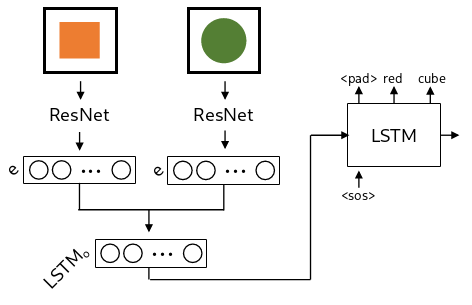
\includegraphics[width=.5\linewidth]{figures/arch_bb_caption_generator.png}
    \caption{Simplified architecture of the bounding box RE generator}
    \label{fig:bb_re_generator_architecture}
\end{figure}

In the first setup, the \textbf{bounding box RE generator}, the model receives the bounding boxes as input (see Figure \ref{fig:bb_re_generator_architecture}).
The first bounding box is always the target object, while the remaining bounding boxes are shuffled.
As in the previous experiment, each bounding box is embedded, using the same \emph{bounding box encoder} submodule: first it is passed through \emph{ResNet-avg} and afterwards projected to an image embedding dimension $e$ with a linear layer.
The \emph{RE generator} submodule uses these embedding to produce a referring expression.
Hereby, all encoded bounding boxes are concatenated and again compressed to the decoder output dimension $LSTM_o$ using another linear layer.
This representation of all objects serves as the initial hidden state of an LSTM, which generates the referring expression.
Tokens used in the LSTM are embedded with embedding dimension $LSTM_e$.
During training, teacher forcing is applied by using embeddings of the ground truth tokens as the input sequence for the LSTM, instead of the output of the LSTM.
The output of the LSTM is passed through a linear layer at each step to determine logits over the symbols of the vocabulary.
During testing, the LSTM is always forced to generate three tokens, with an embedded start-of-sequence token as first input to the LSTM.
Each token in the sequence is determined greedily, by selecting the highest logit in the output of each step in the LSTM.

In the second setup two different models are compared against each other.
The first model, the \textbf{basic RE generator} acts as the baseline and only receives the complete image as the input.
The image is encoded, using the \emph{image encoder} submodule, described in Section \ref{sec:image-processing}, in particular it is passed through \emph{ResNet-3} and subsequently processed by several additional convolution layers.
The same \emph{RE generator} submodule as for the bounding boxes is used to produce the referring expression.
Hereby, since there is only one input scene, its encoding is directly reduced to the decoder output dimension $LSTM_o$.
The LSTM is trained in the same way as above.

\begin{figure}[ht]
    \centering
    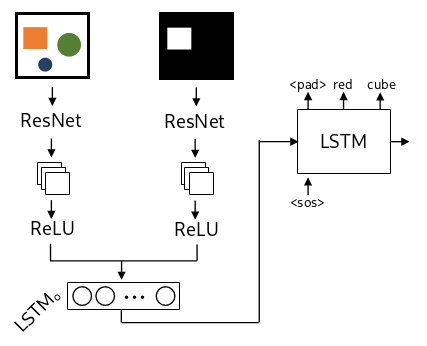
\includegraphics[width=.5\linewidth]{figures/arch_caption_generator.png}
    \caption{Simplified architecture of the masked RE generator}
    \label{fig:masked_re_generator_architecture}
\end{figure}

Using this approach, the model doesn't have any information about the target object and is therefore expected to produce referring expressions for a randomly selected object on the scene.
Therefore, it is extended in a second step with attention to the target object, the \textbf{masked RE generator} (see Figure \ref{fig:masked_re_generator_architecture}).
% SD: You add attention to the target object.
% DK: (added; done)
A masked version of the image is created and passed to the model.
For this, a fixed size squared area of 96 \times\ 96 pixels around the center of the target object is filled in white, while the rest of the image is filled in black.
Both original and masked image are processed together with the \emph{masked image encoder} submodule described in Section \ref{sec:image-processing}.
% SD: This is normally implemented as a filter of 1 and 0 corresponding to pixels. As such it then corresponds to attention, cf. paper with Mehdi.
% DK: (done)
Accordingly, the same \emph{RE generator} submodule is utilized here.
This should point the model towards which object to describe and discriminate from the distractors.

For both setups, the same hyperparameters as in the previous experiments are used: a learning rate of $2\times10^{-4}$, a batch size of 32 samples and 30 epochs, \emph{Adam} \citep{Kingma2015} as optimizer.
8000 randomly selected samples are used for training, the remaining 2000 samples for testing.
The loss is calculated using cross entropy.
Table \ref{tab:variables-reference-expression-generation} shows which variables are compared for each model:

\begin{table}[ht]
    \centering
    \begin{tabular}{lccc}
        \toprule
                                  & $e$                & $LSTM_o$           & $LSTM_e$       \\
                                  & $[100, 500, 1000]$ & $[100, 500, 1000]$ & $[10, 15, 30]$ \\\midrule
        bounding box RE generator & \times             & \times             & \times         \\
        basic RE generator        & -                  & \times             & \times         \\
        masked RE generator       & -                  & \times             & \times         \\
        \bottomrule
    \end{tabular}
    \caption{Variables for each model where $e$ is the embedding dimension, $LSTM_e$ the embedding dimensions for tokens in the LSTM and $LSTM_o$ the output dimension of the LSTM}
    \label{tab:variables-reference-expression-generation}
\end{table}

As already discussed before, this task can be interpreted as a classification task rather than a natural language generation task.
The main reason for this is that the model is tasked to assign specific attributes to the target object instead of producing free text with a large vocabulary.
Following, we are interested in the classification mistakes the model makes.
For this, the model's success is validated on accuracy, recall and precision scores.
These are calculated in the following ways.
The first measure is the \textbf{overall accuracy} if the model predicted every word in the referring expression correctly.
% SD: This is too strict. if this is a generation task then we can use generation metrics. Those compare if the generated string as a whole is kind of similar to the target string, see ROUGE, METEOR, BERTscore.
% If this is a classification task, and it is, given that we know what type of word we expect in each slot, we could calculate accuracy per class, precision, recall, F-score. We could also calculate mean ranks for predicting words per classes, or acucracy at k- if the target word is in the k-top predictions.
% We could also take it a multi-class classification problem and how to calculate accuracy in this case, would need to check.
% DK: I agree that classification metrics refelct success better here (therefore I also used accuracy). These metrics would give a better overview, but I don't think there is time to implement it (QUESTION)
This gives a hint, how the model fares in general and if it is able to predict any of the attributes.
However, a 'false' prediction doesn't give much insight into why the model predicted a wrong referring expression.

It could be the case that the model predicted the correct shape, but wrong color.
Even worse, the model could have predicted more attributes than necessary to uniquely identify the target object and didn't follow the rules of the GRE-algorithm.
For instance, consider the scene in Figure \ref{fig:clevr-dale-5}.
% SD: Too far away, might be worth repeating here, you say still stay Fiigure 2d, repeated asFigure 6 here
% DK: TODO
The correct referring expression is \emph{cylinder}.
If the model would predict \emph{purple cylinder}, the accuracy determines it as false as generating the referring expression \emph{large purple cylinder} as well \emph{small green cube}.
The first two descriptions identify the target object perfectly, but the model only didn't learn to exclude unnecessary attributes.
To mitigate this, the accuracies for each class are included, as well as the macro average.
% SD: Is this figure for a particular class, i.e. object type, or do you then do something to individual accuracy, i.e. average them?
% DK: the metric is averaged over all samples (not by class). Might be definitly worth to do it class by class. Time? (QUESTION)
This can give a better understanding of the errors the model makes.
The same is done for \textbf{precision} and \textbf{recall}.

% SD: Very good If I understand this right this would be a case where the generated description describes another object better than the target and a human would identify that. So it is like false negatives in describing. Perhaps use another term for this: referring to a distractor? (since you are not measuring hwo individually the description fitts a distractor but only if the entire description could perfectly fit a distractor)
% DK: exactly. I added false negatives. But I would like to keep accuracy in the name, since that is what it is. maybe better distractor accuracy? (QUESTION)
With the \textbf{non-target accuracy}, we identify if the model described another object, which is not the target image.
This is basically an inverted accuracy score; the lower the score, the better the model fares.
By this, it measures the false negative generated referring expressions.
For this, referring generations are generated for all the non-target objects and distractors in the images using the GRE-algorithm.
Importantly to notice is that the referring expressions may not uniquely identify a distractor, since multiple distractors with the same shape, color and size are allowed.
If the generated description of the model describes an object that is not the target object, it gets assigned 100\%.
If not, independently of describing the target object, no object, or one of the objects insufficiently, it gets assigned 0\%.
Using this measure, we can get an overview if the model's problem lies in extracting and relating attributes or in understanding which of the presented objects is the target object.

The RE generator models are trained on both 'Dale' datasets.
Again, each of these datasets increases the complexity of the description.
While the referring expression for the \emph{Dale-2} datasets are generally shorter, expressions of the \emph{Dale-5} datasets need to be more specific and use more attributes.
Additionally, the model needs to attend to many more locations in the image at the same time to find discriminating factors between those.
Furthermore, the models are trained on the \emph{CLEVR color} dataset.
In this dataset, the focus lies mainly on only one discriminating attribute, the color.
This might help the model in its prediction and will be tested in the experiments.

\subsubsection*{Results}
Table \ref{tab:results:bb-re-generator} shows the \emph{overall accuracy}, \emph{F1 scores} for each word and the \emph{non-target accuracies} of the \textbf{bounding box RE generator} when trained on the \emph{Dale-2}, \emph{Dale-5} and \emph{CLEVR color} datasets.
As can be seen, the overall accuracies, in other words perfect matches of the generated referring expression depend very much on the dataset.
With the \emph{Dale-2} dataset, the model can achieve perfect matches in 99\% of the cases in its best configuration.
Also the \emph{CLEVR color} dataset allows the model to predict the correct referring expression in 93\% of the samples.
Opposed to that the model can only generate perfect referring expressions in 69\% of the samples of the \emph{Dale-5} dataset.
Looking at the \emph{non-target accuracy}, one of the problems can be identified for the \emph{CLEVR color} dataset.
Summing the \emph{non-target accuracy} and the \emph{overall accuracy}, one gets the accuracy that any of the shown object was described independently if it was the target object.
For the \emph{CLEVR color} dataset, this score lies at 96\% to 97\% in the best configurations, which means that the model described a shown object for almost all the samples.
In 3\% to 4\% of the cases, the model only picked the wrong object to describe.
This looks different for the \emph{Dale-5} dataset.
Here, the model describes only in 71\% of the cases one of the shown objects, 69\% the target object and 2\% a distractor.
The model therefore struggles more with the correct generation of words than with choosing, which object to describe.

When looking at the different configurations, in especially different values for $e$, $LSTM_o$ and $LSTM_e$, it can be seen that the results are not very different for the \emph{Dale-2} and \emph{CLEVR color} datasets.
However, bigger effects can be identified for the \emph{Dale-5} dataset.
Here, a low output dimension of the LSTM $LSTM_o$ tends to give lower scores.
This especially enhanced, when also the embedding dimensions of the tokens $LSTM_e$ is low.
Again, the image embedding size $e$ doesn't seem to have a big effect, when over 50 dimensions.
Indeed, the model achieves an accuracy of 69\% with all three tested embedding sizes.

\begin{table}[ht]
    \centering
    \begin{tabular}{ccc|ccc|ccc|ccc}
        \toprule
               &          &          & \multicolumn{3}{c}{\textbf{Dale-2}} & \multicolumn{3}{c}{\textbf{Dale-5}} & \multicolumn{3}{c}{\textbf{CLEVR color}}                                                                                               \\\cmidrule(lr){4-6}\cmidrule(lr){7-9}\cmidrule(lr){10-12}
        $e$    & $LSTM_o$ & $LSTM_e$ & \textbf{Acc.}                       & \textbf{F1}                         & \textbf{NT}                              & \textbf{Acc.} & \textbf{F1}    & \textbf{NT} & \textbf{Acc.} & \textbf{F1}    & \textbf{NT} \\\midrule
        {100}  & {100}    & {10}     & {97}                                & {97,67}                             & {1}                                      & {65}          & {88,17}        & {2}         & {92}          & {94,95}        & {3}         \\
        {100}  & {100}    & {15}     & {97}                                & {97,77}                             & {0}                                      & {62}          & {86,51}        & {2}         & {92}          & {94,45}        & {4}         \\
        {100}  & {100}    & {30}     & {98}                                & {97,81}                             & {1}                                      & {65}          & {87,97}        & {2}         & {92}          & {94,47}        & {4}         \\
        {100}  & {500}    & {10}     & {98}                                & {98,16}                             & {0}                                      & {67}          & {88,13}        & {2}         & {93}          & {95,18}        & {4}         \\
        {100}  & {500}    & {30}     & \textbf{99}                         & \textbf{98,57}                      & \textbf{0}                               & \textbf{69}   & \textbf{89,53} & \textbf{2}  & \textbf{93}   & \textbf{95,17} & \textbf{3}  \\
        {100}  & {1000}   & {10}     & {98}                                & {98,28}                             & {0}                                      & {68}          & {88,23}        & {2}         & \textbf{93}   & \textbf{95,41} & \textbf{3}  \\
        {500}  & {1000}   & {30}     & \textbf{99}                         & \textbf{98,85}                      & \textbf{0}                               & \textbf{69}   & \textbf{89,15} & \textbf{2}  & {93}          & {95,05}        & {4}         \\
        {500}  & {500}    & {10}     & \textbf{99}                         & \textbf{98,71}                      & \textbf{0}                               & {67}          & {88,99}        & {2}         & \textbf{93}   & \textbf{95,4}  & \textbf{3}  \\
        {1000} & {100}    & {10}     & {97}                                & {97,72}                             & {0}                                      & {59}          & {85,43}        & {2}         & {93}          & {95,04}        & {4}         \\
        {1000} & {100}    & {30}     & {98}                                & {98,16}                             & {0}                                      & {61}          & {86,77}        & {2}         & {92}          & {94,68}        & {4}         \\
        {1000} & {1000}   & {10}     & \textbf{99}                         & \textbf{98,95}                      & \textbf{0}                               & \textbf{69}   & \textbf{89,21} & \textbf{2}  & {93}          & {95,15}        & {4}         \\
        {1000} & {1000}   & {15}     & {99}                                & {98,67}                             & {0}                                      & {68}          & {88,98}        & {2}         & {93}          & {95,01}        & {4}         \\
        \bottomrule
    \end{tabular}
    \caption{Overall accuracies (Acc.), F1-Score (F1) and non-target accuracies (NT) in \% of the bounding box RE generator after 30 epochs: $e$ are different embedding sizes, $LSTM_o$ are different LSTM output sizes and $LSTM_e$ are different embedding sizes for the tokens in the LSTM.}
    \label{tab:results:bb-re-generator}
\end{table}

Tables \ref{tab:results:bb-re-generator_size-shape} and \ref{tab:results:bb-re-generator_color} give a more detailed insight in the results and especially what mistakes the model is making for both the \emph{Dale-5} and \emph{CLEVR color} datasets.
They list \emph{precision} and \emph{recall} metrics for each token for the best configuration of the model with $e=100$, $LSTM_o=500$ and $LSTM_e=30$.
The tokens are grouped by attribute and also show the metrics averaged over each of the attributes.
Since the overall results for the \emph{Dale-2} dataset are already close to perfect, the focus for this analysis lies on the remaining two datasets.
The metrics of the \emph{<pad>} token indicate if the model produced the correct length of the referring expression, in other words if it was able to determine which attributes are necessary to discriminate the target object from the distractors.
For the \emph{CLEVR color} dataset, the scores are perfect.
This is not surprising, because all referring expressions for the \emph{CLEVR color} dataset consist of exactly two attributes, shape and color, and the first generated token will always be the only \emph{<pad>} token in the referring expression (corresponding to the unspecified size).
The \emph{<pad>} token is therefore easy to learn.
For the \emph{Dale-5} dataset, the model struggles more to predict the correct length of the referring expression.

When looking at the tokens for the shape, it can be seen that the model is able to identify it very well across all datasets.
The model predicts the correct shape for all samples using the \emph{CLEVR color} dataset, while both \emph{precision} and \emph{recall} lie around 98,3\% when using the \emph{Dale-5} dataset.
Even though the score is almost perfect, the slight difference might stem from the fact that all distractors have the same shape in the first case, while distractors can be different in the second case.
Consequently, the model is only exposed to one shape at a time for each sample, which might simplify its identification.

For the color attribute, the metrics drop significantly for both \emph{Dale-5} and \emph{CLEVR color} to an average of around 93\%.
Hereby, no meaningful difference can be seen across the datasets, but there are differences between the colors.
Some colors are predicted with \emph{precision} and \emph{recall} around 95\% to 96\%, while others are only around 90\%.
However, these differences are not reproducible across multiple runs and configurations.
The best and worst predicted colors vary and no conclusions can be drawn which colors are easier to predict for the model.

Finally, the size is the most difficult attribute to predict for the model.
Apart from the \emph{CLEVR color} dataset, where a size never needs to be predicted and also is never predicted, the metrics for the prediction of size tokens are the lowest across all tokens.
They are the only mistakes, the model makes, when exposed to the \emph{Dale-2} dataset and the average \emph{precision} lies around 23\% below the average of predictions of the color for the \emph{Dale-5} dataset, while the average \emph{recall} lies around 28,82\% below.
The reason why the \emph{precision} is higher than the \emph{recall} is the \emph{<pad>} token, which is predicted very often instead of a token specifying the size.
In fact, the opposite relationship is visible for the \emph{precision} and \emph{recall} for said token.
The much higher absolute number of \emph{<pad>} tokens leads to a smaller relative difference of \%-points shown in the table.
Again, no conclusion can be drawn if larger or smaller objects are easier to predict, since the results vary across runs and configurations.

\begin{table}[ht]
    \centering
    \begin{tabular}{rr|cc|c|ccc|c|c}
        \toprule
                                         &             & {small} & {large} & \textbf{size}  & {cube}  & {cylinder} & {sphere} & \textbf{shape} & {<pad>} \\\midrule
        \multirow{2}{*}{\textbf{Dale-2}} & {Precision} & {99,17} & {98,29} & \textbf{98,73} & {99,86} & {99,71}    & {99,67}  & \textbf{99,75} & {99,64} \\
                                         & {Recall}    & {97,54} & {94,26} & \textbf{95,9}  & {100}   & {99,56}    & {99,67}  & \textbf{99,74} & {99,77} \\\midrule
        \multirow{2}{*}{\textbf{Dale-5}} & {Precision} & {69,65} & {69,21} & \textbf{69,43} & {98,19} & {98,32}    & {98,39}  & \textbf{98,3}  & {82,22} \\
                                         & {Recall}    & {62,11} & {66,15} & \textbf{64,13} & {98,79} & {97,87}    & {98,25}  & \textbf{98,3}  & {84,59} \\\midrule
        \multirowcell{2}[0pt][r]{\textbf{CLEVR}                                                                                                          \\\textbf{color}} & {Precision}  & {-}     & {-}     & \textbf{-}     & {100}   & {100}      & {100}    & \textbf{100}   & {100}   \\
                                         & {Recall}    & {-}     & {-}     & \textbf{-}     & {100}   & {100}      & {100}    & \textbf{100}   & {100}   \\
        \bottomrule
    \end{tabular}
    \caption{Precision and Recall in \% for <pad>, size and shape tokens with $e=100$, $LSTM_o=500$ and $LSTM_e=30$. The columns \textbf{shape} and \textbf{size} show the average across all tokens of the respective attribute.}
    \label{tab:results:bb-re-generator_size-shape}
\end{table}

\begin{table}[ht]
    \centering
    \begin{tabular}{rr|cccccccc|c}
        \toprule
                                         &             & {blue}  & {brown} & {cyan}  & {gray}  & {green} & {purple} & {red}   & {yellow} & \textbf{color} \\\midrule
        \multirow{2}{*}{\textbf{Dale-2}} & {Precision} & {94,51} & {98,77} & {97,59} & {98,68} & {98,89} & {98,8}   & {97,47} & {100}    & \textbf{98,09} \\
                                         & {Recall}    & {97,73} & {100}   & {98,78} & {97,4}  & {96,74} & {98,8}   & {100}   & {98,8}   & \textbf{98,53} \\\midrule
        \multirow{2}{*}{\textbf{Dale-5}} & {Precision} & {92,12} & {93,82} & {89,13} & {89,12} & {92,63} & {91,12}  & {97,24} & {94,36}  & \textbf{92,44} \\
                                         & {Recall}    & {92,12} & {89,78} & {94,91} & {94,51} & {95,71} & {92,42}  & {89,34} & {94,85}  & \textbf{92,95} \\\midrule
        \multirowcell{2}[0pt][r]{\textbf{CLEVR}                                                                                                           \\\textbf{color}} & {Precision}           & {93,46} & {92,37} & {94,47} & {93,86} & {92,04} & {91,13}  & {90,07} & {94,7}   & \textbf{92,76} \\
                                         & {Recall}    & {92,75} & {92}    & {95,98} & {89,92} & {94,12} & {91,13}  & {94,23} & {91,91}  & \textbf{92,76} \\
        \bottomrule
    \end{tabular}
    \caption{Precision and Recall in \% for color tokens with $e=100$, $LSTM_o=500$ and $LSTM_e=30$. The column \textbf{color} shows the average across all colors.}
    \label{tab:results:bb-re-generator_color}
\end{table}

The approach, how the padding is produced and in which order the attributes are concatenated didn't have an effect on the described metrics.
When the order was reversed and the padding appended, the model was converging slightly faster and reached the limit around two to three epochs earlier.
The final peak stayed exactly the same and the effects were therefore not studied deeper.
% SD: Earlier you say that you will only try one method but now you have tried both. Change earlier text; also do you have full performance figures for this setup to include?
% DK: where? I can't find it. (QUESTION). Since they are the same (and are therefore not central in this study), i didn't inlcude them. (QUESTION)

In conclusion, it can be said that the model is able to extract discriminative features from the shown bounding boxes and produce referring expressions.
However, the result highly depends on the amount of distractors and the resulting need of more discriminative features to describe the target object.
While the shape is easily identified, the model has bigger problems to identify the color and especially the size of the target object.

In the following paragraphs, the results of the \textbf{basic RE generator} as well as the \textbf{masked RE generator} are evaluated.
Compared to the \emph{bounding box RE generator}, the task differs substantially.
Instead of bounding boxes, the model is shown the image of the whole scene.
In addition to extracting features of the target object and distractors separately, the model is now tasked to extract these at once for all objects.
Furthermore, it needs to learn which of the objects is the target object by combining the image with the masked image.
The \emph{basic RE generator} acts hereby as a baseline.
Since there is no information about the target object present, the model is expected to extract the features of all objects, but not to be able to focus on the target object.
Masking should help the model, to also solve the second task.

\begin{table}[ht]
    \centering
    \begin{tabular}{cc|ccc|ccc|ccc}
        \toprule
                  &           & \multicolumn{3}{c}{\textbf{Dale-2}} & \multicolumn{3}{c}{\textbf{Dale-5}} & \multicolumn{3}{c}{\textbf{CLEVR colour}}                                                                                         \\  \cmidrule(lr){3-5}\cmidrule(lr){6-8}\cmidrule(lr){9-11}
        $LSTM\_o$ & $LSTM\_e$ & \textbf{Acc.}                       & \textbf{F1}                         & \textbf{NT}                               & \textbf{Acc.} & \textbf{F1} & \textbf{NT} & \textbf{Acc.} & \textbf{F1} & \textbf{NT} \\\midrule
        {100}     & {30}      & {38}                                & {41,16}                             & {40}                                      & {14}          & {48,91}     & {34}        & {15}          & {36,98}     & {34}        \\
        {1500}    & {15}      & {45}                                & {62,66}                             & {45}                                      & {17}          & {51,89}     & {38}        & {13}          & {35,85}     & {33}        \\
        {2000}    & {10}      & {45}                                & {60,72}                             & {44}                                      & {16}          & {50,77}     & {37}        & {13}          & {34,96}     & {36}        \\
        \bottomrule
    \end{tabular}
    \caption{Overall accuracies (Acc.), F1-Score (F1) and non-target accuracies (NT) in \% of the basic RE generator after 30 epochs for selected configurations: $LSTM_o$ are different LSTM output sizes and $LSTM_e$ are different embedding sizes for the tokens in the LSTM.}
    \label{tab:results:basic-re-generator}
\end{table}

Table \ref{tab:results:basic-re-generator} shows some selected results for the \emph{basic RE generator} after 30 epochs.
The sum of the \emph{overall accuracy} and \emph{non-target accuracy} represents in how many cases any of the shown objects were described, independently if it is a distractor or the target object.
As can be seen, the sum is always relatively high independently of the dataset.
This shows verifies that the model is able to extract information about the objects in the image.
However, it can't decide which object to describe.
Most clearly, this is shown with the \emph{Dale-2} dataset where the sum lies around 90\%.
In almost all samples, the  model describes an object perfectly, but in 45\% of the cases it is the target object, in 45\% the distractor.
Which object, the model chooses is pure chance.
The same pattern is visible for the other datasets.
Since there are more distractors in the scenes, the model is more likely to describe on of those, when deciding randomly, and the \emph{non-target accuracy} is higher than the \emph{overall accuracy}.
However, another fact plays a role here.
The incremental GRE-algorithm can only generate unique referring expressions, when the referred to object is unique in the scene.
This applies to all target objects, but there is no such restriction on the distractors.
One scene can include for instance multiple \emph{large red spheres} as distractors.
The algorithm then generates two identical referring expressions which can affect the \emph{non-target accuracy}.
Indeed, while the average number of distractors per scene in the \emph{CLEVR color} dataset is 7,5, the average number of unique distractors lies at 2,7.
As seen later, the model learns to correctly never predict a \emph{size} and always predict the correct \emph{shape}.
Given this fact, a random guess of a color would predict in $\frac{1}{8} * 2,7 = 33,9\%$ of the cases a unique distractor while in $\frac{1}{8}=12,5\%$ of the cases it would predict the target object.
This corresponds the \emph{non-target accuracies} and \emph{overall accuracies} the \emph{CLEVR color} dataset.
The high \emph{non-target accuracy} is therefore misleading and doesn't represent that the model identified other objects in the scene.

\begin{table}[ht]
    \centering
    \begin{tabular}{cc|ccc|ccc|ccc}
        \toprule
                 &          & \multicolumn{3}{c}{\textbf{Dale-2}} & \multicolumn{3}{c}{\textbf{Dale-5}} & \multicolumn{3}{c}{\textbf{CLEVR color}}                                                                                               \\  \cmidrule(lr){3-5}\cmidrule(lr){6-8}\cmidrule(lr){9-11}
        $LSTM_o$ & $LSTM_e$ & \textbf{Acc.}                       & \textbf{F1}                         & \textbf{NT}                              & \textbf{Acc.} & \textbf{F1}    & \textbf{NT} & \textbf{Acc.} & \textbf{F1}    & \textbf{NT} \\\midrule
        {100}    & {10}     & {81}                                & {76,16}                             & {9}                                      & {21}          & {57,07}        & {23}        & {16}          & {43,69}        & {31}        \\
        {100}    & {15}     & {78}                                & {72,06}                             & {11}                                     & {17}          & {53,29}        & {25}        & {26}          & {50,87}        & {30}        \\
        {100}    & {30}     & {83}                                & {78,76}                             & {7}                                      & {19}          & {54,91}        & {24}        & \textbf{29}   & \textbf{53,37} & \textbf{26} \\
        {500}    & {10}     & {83}                                & {79,78}                             & {6}                                      & {27}          & {62,05}        & {16}        & {17}          & {44,93}        & {32}        \\
        {500}    & {15}     & {83}                                & {79,75}                             & {7}                                      & {28}          & {63,78}        & {16}        & {21}          & {47,08}        & {31}        \\
        {500}    & {30}     & {84}                                & {83,03}                             & {5}                                      & {30}          & {64,36}        & {17}        & {21}          & {40}           & {31}        \\
        {1000}   & {10}     & {84}                                & {82,2}                              & {5}                                      & {31}          & {65,58}        & {13}        & {12}          & {37,67}        & {34}        \\
        {1000}   & {15}     & {85}                                & {82,62}                             & {5}                                      & {31}          & {64,28}        & {16}        & {16}          & {43,27}        & {32}        \\
        {1000}   & {30}     & {85}                                & {83,13}                             & {4}                                      & {31}          & {64,06}        & {17}        & {13}          & {41,79}        & {34}        \\
        {1500}   & {10}     & {84}                                & {81,27}                             & {4}                                      & {33}          & {67,5}         & {14}        & {12}          & {39,04}        & {34}        \\
        {1500}   & {15}     & \textbf{85}                         & \textbf{84,11}                      & \textbf{4}                               & {35}          & {69,05}        & {12}        & {17}          & {44,98}        & {31}        \\
        {1500}   & {30}     & {84}                                & {80,93}                             & {4}                                      & {36}          & {68,97}        & {15}        & {14}          & {42,99}        & {33}        \\
        {2000}   & {10}     & {83}                                & {82,69}                             & {4}                                      & \textbf{36}   & \textbf{69,11} & \textbf{13} & {13}          & {41,85}        & {34}        \\
        {2000}   & {15}     & {84}                                & {81,95}                             & {4}                                      & {34}          & {66,94}        & {14}        & {14}          & {38,79}        & {33}        \\
        {2000}   & {30}     & {85}                                & {82,8}                              & {4}                                      & {32}          & {65,52}        & {16}        & {18}          & {45,41}        & {32}        \\
        {3000}   & {10}     & {82}                                & {79,83}                             & {4}                                      & {34}          & {67,61}        & {12}        & {12}          & {38}           & {34}        \\
        {3000}   & {15}     & {85}                                & {81,8}                              & {4}                                      & {32}          & {65,64}        & {15}        & {13}          & {38,52}        & {35}        \\
        {3000}   & {30}     & {83}                                & {80,6}                              & {3}                                      & {30}          & {63,5}         & {16}        & {12}          & {38,45}        & {34}        \\
        \bottomrule
    \end{tabular}
    \caption{Overall accuracies (Acc.), F1-Score (F1) and non-target accuracies (NT) in \% of the masked RE generator after 30 epochs: $LSTM_o$ are different LSTM output sizes and $LSTM_e$ are different embedding sizes for the tokens in the LSTM.}
    \label{tab:results:masked-re-generator}
    % SD: Masking does not work but perhaps this is because you applied convolutional pre-trained filters rather than 0-1. It is harder to detect meaningful patterns since the targets will be smaller and more integrated with other objects.
    % DK: might be the case. in the last language game i use only a linear layer instead of convolutions, but it doesn't help. This however might also be due to other problems. Time? (QUESTION, future work)
    % SD: I would present these for individual classes.
    % DK: I only have accuracy scores at. Time? (QUESTION)
\end{table}

Table \ref{tab:results:masked-re-generator} shows the results for the \emph{masked RE generator} after 30 epochs.
A first look at the sum of the \emph{overall accuracy} and the \emph{non-target accuracy} shows the model is able to extract the attributes from the shown objects.
For the \emph{Dale-2} dataset, this number lies at 90\% for the best configuration, at 51\% for the \emph{Dale-5} dataset and at 55\% for the \emph{CLEVR color} dataset.
Those sums correspond more or less to the sums of the model without masking shown in Table \ref{tab:results:basic-re-generator}.
In other words, the masking doesn't hinder the model to extract and describe attributes in the image.
However, the balance in between the two accuracy scores shifts towards the \emph{overall accuracy}, meaning that the model is now able to identify the correct target object more often.
While the model still achieves 85\% \emph{overall accuracy} in its best configuration, for the \emph{Dale-2} dataset, the model only reaches 36\% for the \emph{Dale-5} dataset and 29\% for the \emph{CLEVR color} dataset.
The scores for all datasets are all well above the \emph{basic RE generator} baselines of 45\%, 16\% and 15\% respectively, while in all cases the \emph{non-target accuracies} drop lower.
In other words, the masked image helps the model to focus on the correct object.

Comparing it to the less complex \emph{bounding box RE generator}, the results are much less accurate.
This applies to all datasets, even though it is most apparent for the \emph{CLEVR color} dataset.
Given the highly increased complexity of the task, the model fares well in comparison on the \emph{Dale} datasets.

Moreover, the referring expression generated for the \emph{Dale-2} dataset are also efficient in the sense that they follow the incremental GRE-algorithm and only use necessary discriminative attributes.
Features of both target object and distractor are therefore extracted and associated with the vocabulary.
Striking in these results is also the \emph{non-target accuracy}, which is much higher than for the \emph{bounding box RE generator}.
For the \emph{Dale-2} dataset, it arrives at 11\% in one configuration, for the \emph{Dale-5} dataset, the model describes for at least 12\% of the samples a distractor, for one configuration even in over 25\% of the cases.
The \emph{non-target accuracy} of the \emph{CLEVR color} is misleading, and is therefore not considered.
This shows that the model still struggles to learn which of the objects in the scene is the target object, even though masking is applied.

Looking at the effects of the LSTM output size $LSTM_o$ and the LSTM embedding size $LSTM_e$, a difference between the \emph{Dale} datasets and the \emph{CLEVR color} dataset can be identified.
A higher $LSTM_o$ tends to increase the performance of the model, when presented with the \emph{Dale} datasets until a size of 1500 to 2000 dimensions.
When it is further increased the model starts to perform worse.
Furthermore, with a low $LSTM_o$, the model is more likely to identify and describe a distractor, while a higher $LSTM_o$ helps the model to focus on the target object.
The $LSTM_e$ however doesn't seem to have a big consistent effect on the results. With an $LSTM_o$ of around 1500 to 2000, the model seems to fare slightly better with higher $LSTM_e$ of 15 or 30 dimensions.
For the \emph{CLEVR color} dataset, the results look different.
Opposed to the former datasets, a lower $LSTM_o$ helps the model to describe the correct target object.
On the other side, the \emph{non-target accuracy} stays relatively constant independently of the variables at the same level as for the \emph{basic RE generator}.
This indicates that the model uses random guesses of the color when it is not able to extract the color of the target object.
To confirm this, the model's performance on different tokens and attributes are analyzed.

\begin{table}[ht]
    \centering
    \begin{tabular}{rr|cc|c|ccc|c|c}
        \toprule
                                         &             & {small} & {large} & \textbf{size}  & {cube}  & {cylinder} & {sphere} & \textbf{shape} & {<pad>} \\\midrule
        \multirow{2}{*}{\textbf{Dale-2}} & {Precision} & {68,63} & {76}    & \textbf{72,31} & {98,41} & {98,18}    & {98,92}  & \textbf{98,5}  & {94,77} \\
                                         & {Recall}    & {30,17} & {34,55} & \textbf{32,36} & {98,7}  & {98,33}    & {98,47}  & \textbf{98,5}  & {98,64} \\\midrule
        \multirow{2}{*}{\textbf{Dale-5}} & {Precision} & {49,47} & {57,3}  & \textbf{53,38} & {87,09} & {83,26}    & {84,78}  & \textbf{85,04} & {64,99} \\
                                         & {Recall}    & {24,67} & {26,7}  & \textbf{25,69} & {83,66} & {85,28}    & {86,03}  & \textbf{84,99} & {77,87} \\\midrule
        \multirowcell{2}[0pt][r]{\textbf{CLEVR}                                                                                                          \\\textbf{color}} & {Precision}  & {-}     & {-}     & \textbf{-}     & {100} & {100} & {99,7} & \textbf{99,9} & {100}   \\
                                         & {Recall}    & {-}     & {-}     & \textbf{-}     & {99,85} & {99,85}    & {100}    & \textbf{99,9}  & {100}   \\
        \bottomrule
    \end{tabular}
    \caption{Precision and Recall in \% of <pad>, size and shape tokens in the best configuration for each dataset (marked in bold in Table \ref{tab:results:masked-re-generator}). The columns \textbf{shape} and \textbf{size} show the average across all tokens of the respective attribute.}
    \label{tab:results:masked-re-generator_size-shape}
\end{table}

\begin{table}[ht]
    \centering
    \begin{tabular}{rr|cccccccc|c}
        \toprule
                                         &             & {blue}  & {brown} & {cyan}  & {gray}  & {green} & {purple} & {red}   & {yellow} & \textbf{color} \\\midrule
        \multirow{2}{*}{\textbf{Dale-2}} & {Precision} & {88,89} & {85,9}  & {81,82} & {85,53} & {79,76} & {84,52}  & {87,76} & {87,36}  & \textbf{85,19} \\
                                         & {Recall}    & {89,89} & {83,75} & {87,8}  & {79,27} & {93,06} & {76,34}  & {90,53} & {81,72}  & \textbf{85,3}  \\\midrule
        \multirow{2}{*}{\textbf{Dale-5}} & {Precision} & {69,51} & {72,73} & {73,48} & {66,27} & {63,23} & {64,32}  & {67,98} & {70,76}  & \textbf{68,53} \\
                                         & {Recall}    & {72,43} & {71,29} & {73,48} & {60,77} & {74,6}  & {74,87}  & {71,13} & {73,57}  & \textbf{71,52} \\\midrule
        \multirowcell{2}[0pt][r]{\textbf{CLEVR}                                                                                                           \\\textbf{color}} & {Precision}           & {37,63} & {39,23} & {22,09} & {20,23} & {33,33} & {22,97} & {24,9} & {43,96} & \textbf{30,54} \\
                                         & {Recall}    & {29,44} & {42,68} & {27,48} & {22,22} & {25,44} & {26,53}  & {26,23} & {37,14}  & \textbf{29,64} \\
        \bottomrule
    \end{tabular}
    \caption{Precision and Recall in \% of color tokens in the best configuration for each dataset (marked in bold in Table \ref{tab:results:masked-re-generator}). The column \textbf{color} shows the average across all colors.}
    \label{tab:results:masked-re-generator_color}
\end{table}

Tables \ref{tab:results:masked-re-generator_size-shape} and \ref{tab:results:masked-re-generator_color} shows the precision and recall for each token.
The metrics on the \emph{<pad>} token show that the model always predicts the correct length of the referring expression when presented with the \emph{CLEVR color} dataset.
For the \emph{Dale-2} dataset, the model is able to do this in almost all the cases, while the model struggles the most with the \emph{Dale-5} dataset.
While this was similar to the \emph{bounding box RE generator}, the effect here is amplified.
Furthermore, the easiest attribute to predict is the shape.
Again, the metrics for the \emph{Dale-2} and \emph{CLEVR color} dataset are almost the same, but the model is much less able to predict the correct shape for images from the \emph{Dale-5} dataset with only around 85\%.
Hereby, the precision is the highest for predicting \emph{cubes} and lowest for predicting \emph{cylinders}, but this varies across runs.

The prediction of the color drops very much in comparison.
While the metrics all lied above 90\% for the \emph{bounding box RE generator}, now none of datasets passes this limit.
With the \emph{Dale-2} dataset, the precision and recall lie around 85\%, with the \emph{Dale-5} dataset around 70\% and around 30\% with the \emph{CLEVR color} dataset.
The drop for the 'Dale' datasets is expected, because of the higher complexity of the task, but the model's performance on the \emph{CLEVR color} dataset is much worse.
Only every third prediction is correct.
Hereby, a difference across the colors is visible.
Some colors reach both precision and recall of around 40\%, while others only of only around 20\%.
Again, which color is captured better differs from run to run.
Interesting is also the margin between the precision and recall for the colors 'blue', 'cyan', 'green', 'purple' and 'yellow'.
A low precision and high recall indicates that the model predicts the specific color more often than needed while the opposite indicates that it predicts the color less often than needed.
In particular, 'blue', 'green' and 'yellow' are predicted too often and 'cyan' and 'purple' are predicted too few.

Finally, the size is again the most difficult attribute to predict.
As the \emph{bounding box RE generator}, the \emph{masked RE generator} learns correctly to never predict a size for the \emph{CLEVR color} dataset.
Interestingly is the fact that the recall is low which shows that the model likely predicts a \emph{<pad>} token instead.
This might be due to the fact that the \emph{<pad>} token is very frequent in the size slot across all referring expressions and the model amplified this fact.
Between both sizes, 'large' objects are easier to predict for the model than 'small' objects.
The difference lies for both \emph{Dale} datasets at around 8\%.
However, the precision is still far above a random guess, when used on the \emph{Dale-2} dataset.
Using the \emph{Dale-5} dataset, the precision only lies at around 50\% to 57\%.


% With 21\% of these descriptions being a description of the target object, the model again uses a random guess.
% Interestingly, passing the masked image to the model doesn't help it to identify the correct object.
% The accuracy stays at the same value.
% In contrast, the non-target accuracy is increased by 5\% points.
% The model is more likely to identify a wrong object.
% Furthermore, the word-by-word accuracy increases from 45\% to 54\%.
% This increase is likely due to the fact that the description of the target object often shares some attributes with distractor objects.
% For instance a sample with a target object being a \emph{small red cube} was identified as a \emph{<pad> <pad> cube} when the model didn't receive the masked image.
% When also the masked image is passed to the model, it generates the description \emph{small blue cube}.
% This was the correct description of a distractor and because of the overlap of the attributes, the word-by-word accuracy increased from 33\% to 66\%.
% SD: Not in the table?
% DK: no, because a result of one specific sample (done)


In conclusion, when the model doesn't need to extract the objects from the scene it performs very well.
In this case, it is able to achieve almost perfect results on the \emph{Dale-2} dataset and very good results on the remaining two datasets.
However, using complete scenes impairs the performance highly.
The \emph{overall accuracies} decrease and the \emph{non-target accuracies} increase; the model has more difficulties to focus on the correct object.
The most difficulties the model has with the \emph{CLEVR color} dataset where only the color is a discriminative attribute.
Looking at the attributes, the last slot (shape) is always the easiest to predict, while the first slot (size for the \emph{Dale} dataset and color for the \emph{CLEVR color} dataset) is the most difficult.
This effect is again amplified when the model needs to extract the objects itself instead of being presented with bounding boxes.

There are two main explanations for these results.
First, as already seen in the previous experiments, a bigger number of distractors confuses the model more where to focus on.
In the \emph{Dale-2} dataset, there are only two possibilities, while the four distractors in the \emph{Dale-5} dataset and up to nine distractors in the \emph{CLEVR color} give the model a bigger choice.
Moreover, having only one attribute to discriminate the target object, poses the model with more difficulties.
% SD: But before you argued, rather pesimistically, that having distractors with the same attributes actaully contributes to greater performance as it is moire likely that the correct word is generated. I would only pose this as a very vague hypothesis to be tested, as you conclude now it is also the case that images with simialr distractors are more difficult to describe correctly. Hence, it is by no way given.
% DK: TODO
The second explanation lies in the incremental GRE-algorithm.
For instance using the \emph{Dale-2} dataset, when only two random objects are placed in a scene, a second (or third) attribute to discriminate the objects is only needed, when the shape is the same.
Otherwise, the shape is enough, and the RE is only one word long.
The probability for this lies at 66,6\%.
% SD: Why 66? We have 3 attributes, right, so 33%?
% DK: but that the other attributes are only needed if the shape is the same. The prob. for the shape being different for the second object is 66% (rephrased; done)
For shape and color being enough, the probability lies at 29,2\% and that all three attributes are necessary is 4,1\%.
Opposed to that the probabilities with four distractors as in the \emph{Dale-5} dataset are 19,8\%, 47\% and 33,2\% respectively.
With four distractors the algorithm is much more likely to produce longer referring expressions.
These are harder to learn and generate for the model since it needs to take more extracted attributes into account to discriminate the target object from the distractors.
This is verified by the lower precisions and recalls of the size and color tokens.
Furthermore, the low recall of the size tokens shows that the model produces too short referring expressions too often.
% SD: I think we need individual accuracies per class and also precision, recall and the f-score. If we include the joint accuracy figure when you also need to explain how you avergaed the infividual accuracies.
% DK: time? (QUESTION)
% SD: Not sure. Note that <pad> is a token. The model has to learn when to say <pad> just as any word, hence knowing when not to dewscribe is also trickly.
% DK: true, but <pad> token is probably the most used token in general and therefore a guess of <pad> just by frequency is likely right? (QUESTION)
